\documentclass{sigchi}\usepackage[]{graphicx}\usepackage[]{color}
%% maxwidth is the original width if it is less than linewidth
%% otherwise use linewidth (to make sure the graphics do not exceed the margin)
\makeatletter
\def\maxwidth{ %
  \ifdim\Gin@nat@width>\linewidth
    \linewidth
  \else
    \Gin@nat@width
  \fi
}
\makeatother

\definecolor{fgcolor}{rgb}{0.345, 0.345, 0.345}
\newcommand{\hlnum}[1]{\textcolor[rgb]{0.686,0.059,0.569}{#1}}%
\newcommand{\hlstr}[1]{\textcolor[rgb]{0.192,0.494,0.8}{#1}}%
\newcommand{\hlcom}[1]{\textcolor[rgb]{0.678,0.584,0.686}{\textit{#1}}}%
\newcommand{\hlopt}[1]{\textcolor[rgb]{0,0,0}{#1}}%
\newcommand{\hlstd}[1]{\textcolor[rgb]{0.345,0.345,0.345}{#1}}%
\newcommand{\hlkwa}[1]{\textcolor[rgb]{0.161,0.373,0.58}{\textbf{#1}}}%
\newcommand{\hlkwb}[1]{\textcolor[rgb]{0.69,0.353,0.396}{#1}}%
\newcommand{\hlkwc}[1]{\textcolor[rgb]{0.333,0.667,0.333}{#1}}%
\newcommand{\hlkwd}[1]{\textcolor[rgb]{0.737,0.353,0.396}{\textbf{#1}}}%

\usepackage{framed}
\makeatletter
\newenvironment{kframe}{%
 \def\at@end@of@kframe{}%
 \ifinner\ifhmode%
  \def\at@end@of@kframe{\end{minipage}}%
  \begin{minipage}{\columnwidth}%
 \fi\fi%
 \def\FrameCommand##1{\hskip\@totalleftmargin \hskip-\fboxsep
 \colorbox{shadecolor}{##1}\hskip-\fboxsep
     % There is no \\@totalrightmargin, so:
     \hskip-\linewidth \hskip-\@totalleftmargin \hskip\columnwidth}%
 \MakeFramed {\advance\hsize-\width
   \@totalleftmargin\z@ \linewidth\hsize
   \@setminipage}}%
 {\par\unskip\endMakeFramed%
 \at@end@of@kframe}
\makeatother

\definecolor{shadecolor}{rgb}{.97, .97, .97}
\definecolor{messagecolor}{rgb}{0, 0, 0}
\definecolor{warningcolor}{rgb}{1, 0, 1}
\definecolor{errorcolor}{rgb}{1, 0, 0}
\newenvironment{knitrout}{}{} % an empty environment to be redefined in TeX

\usepackage{alltt}

% Use this command to override the default ACM copyright statement (e.g. for preprints). 
% Consult the conference website for the camera-ready copyright statement.


%% EXAMPLE BEGIN -- HOW TO OVERRIDE THE DEFAULT COPYRIGHT STRIP -- (July 22, 2013 - Paul Baumann)
\toappear{%$^\ast$ All authors contributed equally. \\
Permission to make digital or hard copies of all or part of this work for personal or classroom use is 	granted without fee provided that copies are not made or distributed for profit or commercial advantage and that copies bear this notice and the full citation on the first page. Copyrights for components of this work owned by others than ACM must be honored. Abstracting with credit is permitted. To copy otherwise, or republish, to post on servers or to redistribute to lists, requires prior specific permission and/or a fee. Request permissions from permissions@acm.org. \\
{\emph{L@S'15}}, March 14--15, 2015, Vancouver, Canada. \\
Copyright \copyright~2015 ACM ISBN/14/04...\$15.00. \\
DOI string from ACM form confirmation}
%% EXAMPLE END -- HOW TO OVERRIDE THE DEFAULT COPYRIGHT STRIP -- (July 22, 2013 - Paul Baumann)


% Arabic page numbers for submission. 
% Remove this line to eliminate page numbers for the camera ready copy
\pagenumbering{arabic}


% Load basic packages
\usepackage{balance}  % to better equalize the last page
\usepackage{graphics} % for EPS, load graphicx instead
\usepackage{times}    % comment if you want LaTeX's default font
\usepackage{url}      % llt: nicely formatted URLs
\usepackage{booktabs}
\usepackage{rotating}

% llt: Define a global style for URLs, rather that the default one
\makeatletter
\def\url@leostyle{%
  \@ifundefined{selectfont}{\def\UrlFont{\sf}}{\def\UrlFont{\small\bf\ttfamily}}}
\makeatother
\urlstyle{leo}


% To make various LaTeX processors do the right thing with page size.
\def\pprw{8.5in}
\def\pprh{11in}
\special{papersize=\pprw,\pprh}
\setlength{\paperwidth}{\pprw}
\setlength{\paperheight}{\pprh}
\setlength{\pdfpagewidth}{\pprw}
\setlength{\pdfpageheight}{\pprh}

% Make sure hyperref comes last of your loaded packages, 
% to give it a fighting chance of not being over-written, 
% since its job is to redefine many LaTeX commands.
\usepackage[pdftex]{hyperref}
\hypersetup{
pdftitle={SIGCHI Conference Proceedings Format},
pdfauthor={LaTeX},
pdfkeywords={SIGCHI, proceedings, archival format},
bookmarksnumbered,
pdfstartview={FitH},
colorlinks,
citecolor=black,
filecolor=black,
linkcolor=black,
urlcolor=black,
breaklinks=true,
}

% create a shortcut to typeset table headings
\newcommand\tabhead[1]{\small\textbf{#1}}


% End of preamble. Here it comes the document.
\IfFileExists{upquote.sty}{\usepackage{upquote}}{}
\begin{document}

\title{Attrition in Online Learning: Understanding Persistence and Dropout in Massive Open Online Courses}

\numberofauthors{2}
\author{
  \alignauthor Omitted for blind review\\
  \affaddr{Institution}\\
  \affaddr{Address}\\
  \email{Email}\\
%   \alignauthor Ren\'{e} F. Kizilcec$^\ast$\\
%     \affaddr{Department of Communication}\\
%     \affaddr{Stanford University}\\
%     \email{kizilcec@stanford.edu}\\
%   \alignauthor Sherif Halawa$^\ast$\\
%     \affaddr{Department of Electrical Engineering}\\
%     \affaddr{Stanford University}\\
%     \email{halawa@stanford.edu}\\
}

\maketitle

\begin{abstract}
Persistence and attrition in MOOCs are systematically analyzed using self-report and behavioral data collected from 20879 online learners in 18 courses. Study 1 offers insights into reasons for disengaging from MOOCs and explores relationships with prior behavior and reported intentions. Study 2 is a case study to develop a deeper understanding of attrition in MOOCs by conducting a case study. Targeting online learners who were predicted likely dropouts in a particular course were invited to provide feedback via a survey. (abstract needs work...)
\end{abstract}

\keywords{Online learning, persistence, attrition, dropout, disengagement, massive open online courses, MOOC, psychological factors}

\category{H.5.m.}{Information Interfaces and Presentation (e.g. HCI)}{Miscellaneous}
\category{K.3.1.}{Computers and Education}{Computer Uses in Education}

\section{Introduction}

Educational environments has become increasingly diverse. Traditional schools and universities have a characteristically rigid structure, including instructor-defined---even nationally agreed---syllabi, fixed time schedules, entry requirements, and material costs to enter and exit. Novel institutional structures have been developed to overcome particular constraints. Community colleges, for instance, were created in an attempt to democratize education by offering instruction at a lower cost and by accommodating people with less flexible schedules \cite{goldrick2010challenges}. Distance learning programs intended to deliver education in remote parts of the world and for people who simply could not attend in-person classes. Course materials, including assessments, were delivered through mail (``correspondence education''), radio, television, and eventually the Internet, thereby addressing geographical and time related constraints of traditional instruction \cite{moore1996distance}.

The latest generation of online learning environments, characterized by massive open online courses (MOOCs), has pushed the boundary on the scale of education \cite{waldrop2013campus}. By design, MOOCs provide course materials to millions of people worldwide. This scale could be achieved by pre-recording lectures, designing assessments that can be graded automatically, and by leveraging the momentum of the number of people involved (e.g., to facilitate peer learning or peer grading \cite{kulkarni2013peer,cambre2014talkabout}). Maybe by virtue of their large scale, their prominent instructors, or their adherence to contemporary interface designs, MOOCs rapidly became an online media phenomenon. People would sign up weeks in advance of the course launch date, many of whom would never even enter the course site. And among those who enroll and enter the site, a large proportion tends to only ``sample'' some content and leave again \cite{kizilcec2013deconstructing}. Many of the prototypical behaviors observed in MOOCs \cite{kizilcec2013deconstructing,breslow2013studying} (other?) resemble those on online media platforms, such as YouTube or tumblr. This trend has also been reflected in the diversity of MOOC learners' motivations for enrolling \cite{kizilcec2015motivation}.

Shortly after the first wave of courses had finished, extensive media coverage led to MOOCs becoming associated with high attrition rates \cite{lewin2013after,parr2013mooc,guthrie2013moocs}. Early MOOC research cautioned against dichotomizing learners into successes and failures based on course completion \cite{kizilcec2013deconstructing,rivard2013measuring}. Instead, more nuanced categorizations based on learner behavior \cite{kizilcec2013deconstructing,clow2013moocs} (other?), motivations \cite{kizilcec2015motivation}, or intentions \cite{wilkowski2014student} have been suggested. Ultimately, perspectives on persistence and attrition in MOOCs depend on how MOOCs have been conceptualized. Kizilcec and Schneider \citeyear{kizilcec2015motivation} proposed that MOOCs have bridged two different world: one world is governed by the user-centric norms of online media, where everyone is encouraged to be as active as they wish; the other world adheres to the ``grammar of schooling'', which presupposes instructor-defined goals that students strive to achieve \cite{tyack1994grammar}. Viewing MOOC participation as bridging these two worlds undoubtedly adds a layer of complexity to interpretations of attrition.

This paper presents a systematic investigation into attrition in MOOCs, based on self-report and behavioral data collected from [N] online learners in [M] courses. We begin by briefly reviewing the large literature on attrition in educational environments with a focus on important developments in understanding its causes. Building on this foundation of prior work, Study 1 offers insights into reasons for disengaging from MOOCs and explores relationships with prior behavior and reported intentions. In Study 2, we sought to develop a deeper understanding of attrition in MOOCs by conducting a case study. Targeting around 7,000 online learners who were predicted likely dropouts in a particular course were invited to provide feedback via a survey. 
TODO: complete paragraph based on what we actually do in Study 2.


\section{Related Work}

Research and theorizing on attrition in education has a rich history. This review is intended to serve as a foundation to build on with the current research. We therefore simultaneously develop research questions and hypotheses to investigate and test in the current work. The focus of this brief review is on how ways of thinking about attrition have developed over the last decades. 

\subsection{In-person Education}

The majority of early work on attrition centered around theoretical models of students' decision to persist or dropout of a traditional higher education setting. An early model suggested that students' presistence is largely driven by their prior behavior, attitudes, and norms \cite{fishbein1975belief}. The psychological processes involved in turning an intent to learn into the decision to persist were thought to be mediated by volition, i.e., the extent to which the student engages in goal-direct behaviors in the face of distraction \cite{corno1993role}. Hence, motivation alone is necessary but not sufficient for persistence. Students may fail to sustain efforts in the absence of strong self-regulatory skills.

\begin{description}
  \item[RQ1] How do prior learner characteristics (demographics, geographic location, intentions and motivations, and previous online courses) influence learners' likelihood of dropping out of a MOOC?
  \item[H1] Successful MOOC learners exhibit higher levels of goal striving than unsuccessful ones.
\end{description}

The next generation of psychological models, which were highly influential in the literature, emphasized the critical role of students' ``fit'' in the institution. Tinto's \citeyear{tinto1975dropout} student integration model posited that college students' decision to persist is a function of prior experiences and individual students' characteristics, and experiences during college. While prior experiences and characteristics are fixed, schools can influence the college experience, including the degree of social and academic integration. Tinto operationalized academic and social integration by GPA scores and the frequency of positive interactions with peers and instructors, respectively. This resonates with recent work highlighting the critical role of students' feelings of social belonging in achievement-oriented environments \cite{walton2007question}. 

\begin{description}
  \item[H2] Successful MOOC learners exhibit a greater sense of social belonging than unsuccessful ones.
\end{description}

Tinto's work, which specifically targets traditional college students, prompted universities to be proactive in establishing environments that support student integration. Research on attrition in community college settings reiterates the importance of academic and social integration, but points out that non-persistence could indicate success depending on students' intent---students may leave after accomplishing their goal \cite{bers1991persistence}. Nevertheless, a brief psychological intervention that taught community college students an incremental theory of intelligence (i.e., instilling a growth mindset) was found to halve attrition rates and increase academic achievement \cite{paunesku2012brief}. The results highlight the powerful influence of mindset and caution against overinterpreting non-persistence as an indicator of goal achievement.

\begin{description}
  \item[RQ2] What proportion of learners who dropped out were satisfied with their achievements in the course?
  \item[H3] Successful MOOC learners have a more fluid conception of intelligence (i.e., more of a growth than fixed mindset) than unsuccessful ones.
\end{description}

\subsection{Distance Education and e-Learning}

Distance education, in contrast to traditional in-person education, attracts a different student demographic and typically provides fewer opportunities for social integration. However, students in distance learning programs tend to lead social lives outside of school, maybe working part-time and living with their partner. Building on Tinto's model, Bean and Metzner \citeyear{bean1985conceptual} proposed a conceptual model of persistence that would be more applicable to nontraditional students. Persistence is thought to be a function of background characteristics (e.g., demographics), academic and environmental variables (e.g., study habits, financial resources, work and family obligations), and academic and psychological outcomes (e.g., GPA, satisfaction). The significant change from Tinto's orginal model was the inclusion of environmental variables to account for the added complexity of nontraditional students' lives (see \cite{kember1989longitudinal}, for another adaptation of Tinto's model for distance education).

Rovai \citeyear{rovai2003search}, combining Tinto's and Bean and Metzner's models with factors specific to online learning and pedagogical styles, proposed a composite persistence model specifically for students in online distance education programs. Among other novel factors, Rovai's model acknowledges the critical role of computer literacy in online learning. And yet, while the theoretical models become more developed, they became harder to apply to real-world settings, and hence, the empirical evidence to support them remained sparse. An exploratory study of reasons for attrition suggested the following eight constructs, based on over 1,000 online education students: academic and technical skills, learner motivation, time and support for studies, cost and access to the Internet, and technical problems \cite{muilenburg2005student}. An analysis of student behavior on an online education platform showed that 31\% of variation in achievement could be accounted for by a small set of participation measures \cite{morris2005tracking}.

\subsection{MOOCs}

A survey of over one hundred learners who dropped out of a MOOC showed that the majority indicated having too little time due to work responsibilities, not enough social support inside and outside of the course, and insufficient academic and technical support from the course \cite{gutl2014attrition}. A qualitative analysis of public records, especially forum posts, from 42 MOOCs suggested the following reasons for attrition: lack of time, learner motivation, feelings of isolation, lack of interactivity, insufficient prior knowledge or skills, and hidden costs \cite{khalil2014moocs}. A survival analysis of close to 800 learners who had posted on a MOOC discussion forum suggested that the likelihood of dropout was lower for those who i. actively participated in the first week of the course; ii. served as an authority figure in the community on the forum, and iii. did not engage in a particular subcommunity on the forum \cite{yang2013turn}. In addition, a number of machine learning approaches yielded promising results for early dropout prediction (e.g. \cite{taylor2014likely,halawa2014dropout}), but fell short of offering insights into why a given learner would leave the course.

\begin{description}
\item[RQ3a] What reasons do learners report for dropping out of a MOOC?
\item[RQ3b] How do reasons for dropping out vary across prior learner characteristics (cf. RQ1)?
\item[RQ4] How does behavior in MOOCs vary by reasons for dropping out?
\end{description}  

\section{Study 1: Reasons for Disengaging}

% \begin{description}
%   \item[H1] prior experience -- technical difficulties
%   \item[H2] demographics (education) -- course difficulty
% \end{description}


\subsection{Methods}

% Which courses did we use? What data
Seventeen MOOCs on topcis in a variety of disciplines were selected for investigation: four on topics in the humanities, two in engineering, three in computer science, two runs of the same course in business, and six in mathematics and statistics. For each course, we merged data from the course survey (distributed in the first weeks of the course), the feedback surveys (distributed in the last weeks of the course), and behavioral data collected in the learning environment. Only those learners who completed the feedback survey were included in the analyses (some did not complete the initial course survey). Table \ref{tab:study1_courses_summary} provides the following summary statistics for each course: the number of enrolled learners, the number of learners who completed the course survey and the feedback surveys, age, gender, and education level, and the proportion of learners who self-reported that they stopped participating in the course. We also computed the proprtions of learners who viewed at least 30, 50, and 80\% of the course videos.

%Table:  course name; enrollment; pre-survey response rate; prop. demographics (age, gender, educ); who intended to do all; post-survey response rate; self-identified dropout rate
  
\begin{table*}
\label{tab:study1_courses_summary}
\caption{Summary statistics of 14 MOOCs}
\small
\center
\begin{tabular}{llcccccccccc}
\toprule
%  & Topic Area & Enrollment & Course survey & Feedback survey & Female & Age & Education & \specialcellcentered{\ensuremath{>} 30\% \\ videos} & \specialcellcentered{\ensuremath{>} 50\% \\ videos} & \specialcellcentered{\ensuremath{>} 80\% \\ videos} & \specialcellcentered{Self-Rep. \\ Dropout} \\
& & & & & & & & $>$ 30\% & $>$ 50\% & $>$ 80\% & Self-Rep. \\
& Topic Area & Enrollment & Course survey & Feedback survey & Female & Age & Education & videos & videos & videos & Dropout \\
\midrule
C1 & Business & 61,096 & 9,943 & 2,367 & 42\% & 39 (30,49) & n/a & 39\% & 20\% & 7\% & 10\% \\
C2 & Business & 41,081 & 6,544 & 883 & 40\% & 39 (30,49) & 97\% & 32\% & 13\% & 2\% & 9\% \\
C3 & CS & 27,104 & 6,104 & 2,854 & 35\% & 30 (22,41) & 74\% & 67\% & 40\% & 7\% & 2\% \\
C4 & CS & 56,154 & 3,406 & 1,123 & 11\% & 33 (27,42) & 91\% & 34\% & 16\% & 11\% & 21\% \\
C5 & CS & 57,636 & 5738 & 402 & 17\% & 33 (26,43) & 91\% & 66\% & 55\% & 28\% & 14\% \\
C6 & Engineering & 16,220 & 2,540 & 269 & 13\% & 33 (27,45) & 92\% & 62\% & 49\% & 17\% & 15\% \\
C7 & Enginerring & 7,178 & 1,312 & 202 & 12\% & 27 (22,39) & 85\% & 51\% & 18\% & 2\% & 7\% \\
C8 & Humanities & 7,634 & 3,631 & 152 & 92\% & 33 (26,45) & 93\% & 45\% & 11\% & 0\% & 7\% \\
C9 & Humanities & 6,475 & 3,315 & 326 & 90\% & 32 (27,47) & 91\% & 69\% & 50\% & 17\% & 16\% \\
C10 & Humanities & 9,903 & 4,227 & 1,570 & 52\% & 39 (29,52) & 89\% & 84\% & 74\% & 21\% & 3\% \\
C11 & Humanities & 630 & 167 & 80 & 50\% & 30 (27,40) & 97\% & 74\% & 55\% & 16\% & 16\% \\
C12 & Math \& Stats & 49,317 & 3,090 & 862 & 33\% & 41 (29,55) & 88\% & 27\% & 10\% & 1\% & 31\% \\
C13 & Math \& Stats & 32,006 & 26,142 & 5,336 & 58\% & 28 (16,46) & n/a & 69\% & 38\% & 8\% & 4\% \\
C14 & Math \& Stats & 16,857 & 2,892 & 363 & 9\% & 31 (26,38) & 99\% & 61\% & 45\% & 25\% & 14\% \\
C15 & Math \& Stats & 37,017 & 11,629 & 1,854 & 20\% & 35 (29,45) & 98\% & 78\% & 67\% & 34\% & 8\% \\
C16 & Math \& Stats & 27,236 & 2,711 & 637 & 82\% & 43 (34,51) & n/a & 64\% & 36\% & 5\% & 1\% \\
C17 & Math \& Stats & 13,132 & 3,629 & 843 & n/a & n/a & n/a & 70\% & 54\% & 14\% & 5\% \\
\bottomrule
\end{tabular}
\end{table*}



% What LMS data variables did we compute?
We are interested in exploring correlations between reasons for dropout and learner behaviors. If such correlations exist, they can be an additional towards understanding why learners engage with or disengage from various learning activities. In this study, we computed the fraction of videos watched by each learner, fraction of problems attempted, average grade scored on attempted problems, and number of forum posts and replies posted.

\subsection{Results}

%Table: proportions for each dropout reason for each course
\begin{knitrout}
\definecolor{shadecolor}{rgb}{0.969, 0.969, 0.969}\color{fgcolor}\begin{figure*}[ht]

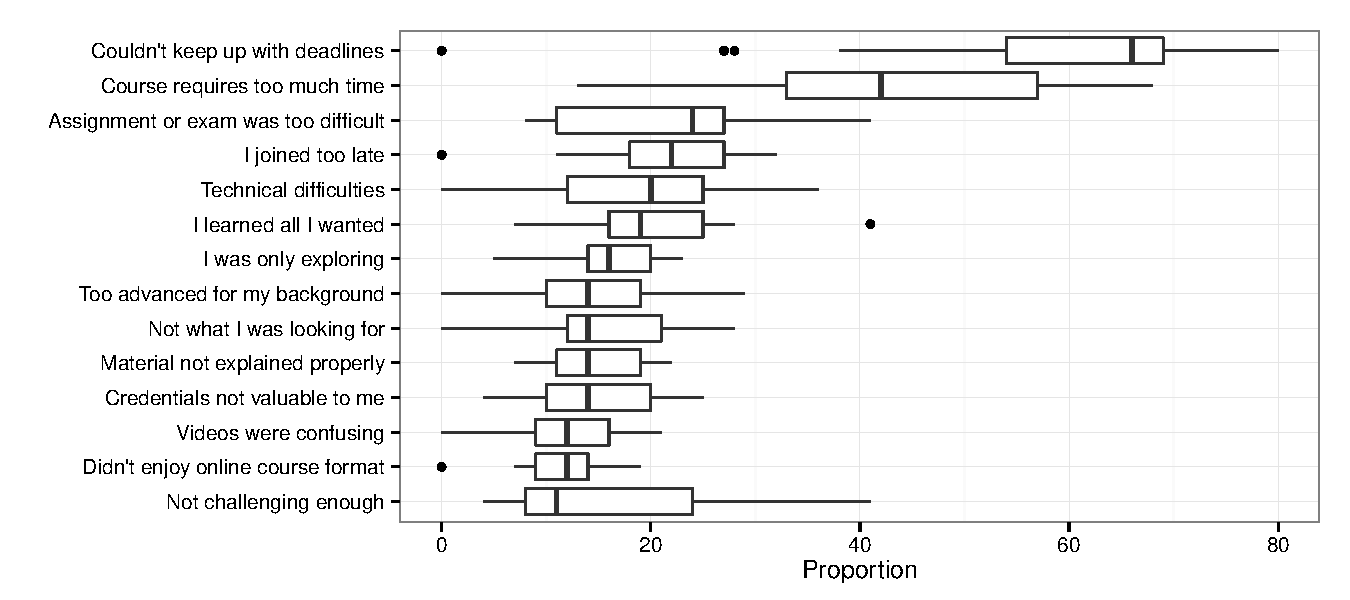
\includegraphics[width=\maxwidth]{figure/prop-reason} \caption[Proportion of learners who indicated each reason for attrition across 17 MOOCs]{Proportion of learners who indicated each reason for attrition across 17 MOOCs\label{fig:prop-reason}}
\end{figure*}


\end{knitrout}

% \begin{sidewaystable}
% \label{tab:proprtion_reason_for_dropout}
% \caption{Distribution of reported reasons for dropping out across courses. Percentage of learners who selected each reason for dropping out in each course, and median and interquartile range across courses}
% \small
% \center
% \begin{tabular}{llrrrrrrrrrrrrrrrrrr}
% \toprule
% Reason for dropout & C1 & C2 & C3 & C4 & C5 & C6 & C7 & C8 & C9 & C10 & C11 & C12 & C13 & C14 & C15 & C16 & C17 & Median & IQR \\
% \midrule
% \specialcellleft{Material not explained \\ properly} & 18 & 20 & 10 & 22 & 19 & 21 & 8 & 11 & 13 & 13 & 9 & 7 & 14 & 18 & 11 & 14 & 19 & 14 & 8 \\
% \specialcellleft{Course requires too \\ much time} & 57 & 39 & 13 & 48 & 42 & 51 & 33 & 60 & 65 & 42 & 18 & 52 & 21 & 68 & 39 & 28 & 68 & 42 & 24 \\
% \specialcellleft{Not what I was looking \\ for} & 21 & 23 & 25 & 14 & 13 & 19 & 8 & 0 & 0 & 23 & 9 & 12 & 20 & 20 & 13 & 28 & 12 & 14 & 9 \\
% I joined too late & 32 & 18 & 25 & 28 & 32 & 28 & 25 & 11 & 20 & 27 & 27 & 19 & 19 & 22 & 18 & 0 & 11 & 22 & 9 \\
% \specialcellleft{Didn't enjoy online \\ course format} & 15 & 14 & 8 & 16 & 13 & 12 & 0 & 0 & 9 & 10 & 9 & 9 & 19 & 12 & 7 & 14 & 14 & 12 & 5 \\
% Technical difficulties & 21 & 3 & 18 & 12 & 17 & 24 & 25 & 30 & 30 & 10 & 36 & 13 & 20 & 25 & 12 & 0 & 21 & 20 & 13 \\
% \specialcellleft{Couldn't keep up with \\ deadlines} & 69 & 58 & 38 & 76 & 80 & 66 & 66 & 55 & 69 & 67 & 27 & 71 & 28 & 64 & 54 & 0 & 71 & 66 & 15 \\
% Not challenging enough & 12 & 7 & 27 & 8 & 4 & 18 & 41 & 11 & 6 & 10 & 27 & 10 & 24 & 14 & 11 & 28 & 7 & 11 & 16 \\
% I learned all I wanted & 18 & 7 & 26 & 17 & 19 & 16 & 41 & 10 & 9 & 25 & 18 & 21 & 27 & 25 & 20 & 28 & 12 & 19 & 9 \\
% Videos were confusing & 13 & 12 & 10 & 19 & 19 & 21 & 0 & 11 & 7 & 13 & 9 & 9 & 11 & 16 & 9 & 14 & 19 & 12 & 7 \\
% I was only exploring & 16 & 5 & 22 & 17 & 14 & 21 & 16 & 11 & 7 & 18 & 20 & 16 & 23 & 20 & 16 & 16 & 12 & 16 & 6 \\
% \specialcellleft{Too advanced for my \\ background} & 14 & 10 & 10 & 23 & 24 & 16 & 8 & 11 & 2 & 13 & 18 & 19 & 10 & 25 & 17 & 0 & 29 & 14 & 9 \\
% \specialcellleft{Assn or exam was too \\ difficult} & 26 & 8 & 11 & 27 & 23 & 39 & 33 & 11 & 24 & 11 & 27 & 27 & 11 & 35 & 15 & 14 & 41 & 24 & 16 \\
% \specialcellleft{Credentials not valuable \\ to me} & 14 & 9 & 18 & 10 & 10 & 18 & 25 & 22 & 4 & 5 & 18 & 7 & 20 & 22 & 14 & 14 & 25 & 14 & 10 \\
% \bottomrule
% \end{tabular}
% \end{sidewaystable}

Table: correlations between reasons and one with cors between reasons and intentions

Plot: ecdf curves for proportion videos watched for each disengagement reason


\subsection{Discussion}


\section{Study 2: Understanding Disengagement}

To gain a better understanding of the attrition patterns identified in Study 1, we designed a smaller, more focused follow-up study. In Study 2, we reached out to learners who were likely to drop out of a course and asked them to provide feedback. To this end, we developed a predictive model to identify at-risk learners and asked them to complete a survey. One goal of this study was to further investiage research question $RQ3a$ about reasons for attrition based on learners' own descriptions of the challenges they faced. Specifically, in Study 1, most learners reported that they disengaged due to a shortage of time. A variety of factors can influence the amount of time learners have at their disposal. Higher priority obligations, such as professional, academic, and personal committments, are certainly large contributors. Another critical factor, especially in the context of MOOCs as largely unguided learning environments, is learners' volitional control to engage in self-regulated learning \cite{corno2001volitional}. For instance, learners' ability to allocate time for the course in the presence of potential distractors of subjectively lower importance than taking the course (e.g., watching TV). We constructed the following hypotheses about the presence of these two factors for learners who report having not enough time:

\begin{description}
  \item[H4a] Learners who report having `not enough time' can be grouped into those with higher priority obligations (professional, academic, and personal) and those with low volitional control.
  \item[H4b] Learners who do not report specific higher-priority obligations tend to exhibit lower volitional control than those who specify particular obligations.
\end{description}  

Another goal of Study 2 was to collect data to test hypotheses $H1, H2,$ and $H3$ on the role of goal striving, social belonging, and growth mindset in the success of MOOC learners. To this end, we included a self-report measures for each construct in the survey that was sent to at-risk learners.

\subsection{Methods}

The particular MOOC under observation was an undergraduate level course on an advanced topic in computer science. It was offered in 2014 through Coursera. There were  20,048 enrolled learners; 10,510 watched at least one video, and [N] attempted more than one assignment.

\subsubsection{Predicting Disengagement}

The objective was to build an `early warning' prediction model that could flag learners who are likely to drop out in the future. We defined the following three criteria by which to evaluate the performance of the model.

\textit{Prediction accuracy}: Prediction recall (the fraction of correctly predicted dropouts) should be high to deliver the survey to as many future dropouts as possible. The false positive rate (the fraction of non-dropouts incorrectly predicted as droputs) should be low to avoid sending a survey to learners who do not experience challenges in the courses.

\textit{Prediction lag}: The period between a learner's last site activity and the time they are flagged as being likely to drop out should be short. A shorter prediction lag improves the likelihood of successfully intervening to help the learner get back on track.

\textit{Transferability}: Whether or not a learner drops out of the course can not be determined before the end of the course. We thus had to train the prediction model using data from previous courses. The performance of the prediction model should be adequate in courses other than those on which it was trained.

The training set was composed of learners' interaction data (predictors) and dropout states (outcome) from 20 MOOCs. The large number of courses should improve model transferability by favoring features that are strongly predictive across different courses. Five hundred learners from each MOOC were included in the training set ($train$), and 500 other learners from the same MOOCs were selected for the first test set ($test_1$). A second test set of similar size was composed from 20 other MOOCs ($test_2$). Features extracted from the interaction data included different aspects of learners' video, assignment, and forum activity; their pace of viewing videos relative to the course pace, as well as various aspects of engagement time, such as the last time the learner interacted with the course (see \cite{halawa2014dropout}, for additional details on the prediction model). The model was fit by logistic regression. Table \ref{tab:drop_pred_rocs} provides information on the prediction performance, measured by the area under the ROC curve (AUC).

\begin{table}[h!]
\caption{Performance of the dropout prediction model}
\label{tab:drop_pred_rocs}
\small
\center
\begin{tabular}{lccc}
\toprule
 & $train$ & $test_1$ & $test_2$ \\
\midrule
AUC &  0.931 & 0.929 & 0.922  \\
\bottomrule
\end{tabular}
\end{table}

Two of the predictors in the fitted model are highly influential. The first is the number of days since the learner has last been active ($x_{1}$). The likelihood that the learner drops out increases substantially if the learner disengages for 14 days or more. However, the likelihood of such a learner re-engaging increases with the fraction of released videos the learner has viewed ($x_{2}$) prior to the absence; this is the second most influential feature in the model. Equation 1 is an approximation of the model with only these two predictors. A learner was flagged if their dropout probability exceeded a half:

\begin{equation}
Pr(\text{dropout}) = \frac{1}{1+e^{-0.431x_1 + 6.388x_2 + 1.626}} > 0.5
\end{equation}

Out of the 20,048 enrolled learners in the course, we only considered those 10,510 who watched at least one lecture video, and 6,074 of them were flagged as likely to drop out. The survey was sent out to 6,053 leaners (excluding 21 learners with invalid email addresses or duplicate accounts).


\subsubsection{Feedback Survey}

Every learner who was predicted to disengage from the course was sent an email kindly requesting their help: ``You are enrolled in [course name], but you've been less active recently. Could you help us understand why?'' A low response rate was expected for this subpopulation that was defined by low engagement. And yet, 756 out of 6,053 learners started the survey (12.5\% response rate), and 459 completed it (61\% completion rate). Missing values were multiply imputated by predictive mean matching using responses to all survey questions.\footnote{The $R$ mice package was used to perform multiple imputation and subsequent pooled analyses.} All estimates were pooled across ten imputations, with standard errors adjusted for added variance. The majority of respondents were male (85\%), 35.6 years old on average ($SD=12.5$), and 80\% had achieved a bachelors' or more advanced degree.

Learners were asked to report how satisfied they were with their progress in the course, and whether they were using the course materials more, less, or exactly as much as they would have liked. These items served as measures of personal success.
% In addition, they reported intentions for engaging with each week's course content. 
They were then asked to openly report ``what challenges, inside or outside of the course, [they] experienced while [they were] taking this course, if any?'' The instructions encouraged them to list all challenges they could think of. This question was deliberately asked prior to any survey questions that could suggest particular reasons for disengagement.

Two research assistants independently developed codebooks for the resulting 448 non-empty open responses. Their codebooks were consolidated and applied on Mechanical Turk in three iterations. The codebook was updated in each iteration to reliably fit the open response data. Specific updates to the initial codebook were informed by code frequency, code correlations, and inter-coder agreement. In the first iteration, 250 randomly selected responses were each coded by four `classification experts'. In the second iteration, the remaining responses were coded in the same way. In the final iteration, all responses were coded by two classification experts (ties were resolved by two researchers).\footnote{For additional details on the coding procedure and codebooks, see [URL].} The iterative coding yielded 399 relevant coded responses, which were analyzed in combination with the remaining survey data.

% Learners also rated the extent to which their progress was hindered by a number of obstacles. 
Learners also rated their sense of social and academic fit \cite{walton2007question} (17 items, $M=4.66, SD=0.71, \alpha=0.86$); mindset (4 items on the nature of intelligence and talent\footnote{Items were adpated from the mindset questionnaire available at \url{http://mindsetonline.com/testyourmindset/}.}; $M=4.44, SD=0.92, \alpha=0.77$), goal striving (4 items on motivation, perceived importance, committment, and confidence; $M=3.12, SD=0.95, \alpha=0.82$), and capacity for volitional control (one item about lower-priority distractions hindering the learner's course progress; $M=2.73, SD=1.29$).

\subsection{Results}

% \subsubsection{Predicting Likely Dropouts}

% SHERIF TODO: Add results of prediction. How well did the prediction work? And who took the survey; how sure was the model that those who took the survey would actually drop out, relative to those who didn't take the survey?

\subsubsection{Reasons for Dropout}

The majority of survey respondents (550 of 756; 73\%) reported being only somewhat or less satisfied with their progress in the course. While many of them (66\%) were substantially held back by other committments that took up time they had planned to spend on the course, only one in four (25\%) indicated being hindered by distractions of lower priority than the course (i.e. exhibit lower volitional control). These two time-related measures, which only differ in the assigned level of priority, were not significantly correlated ($r=.05, t_{548}=1.3, p=.21$).

Reasons for learner attrition were measured using iteratively coded open responses ($n=399$). Table \ref{tab:s2reas} provides each coded challenge and percentage of open responses that indicated it. A number of significant correlations between these challenges stood out: having not enough time was negatively associated with disliking the format or teaching style ($r=-.52$), needing additional course materials ($r=-.26$), finding the course uninteresting or not valuable ($r=-.45$), and facing technical difficulties ($r=-.29$). 

\begin{table}[h!]
\caption{Iteratively-Coded Reasons for Attrition}
\label{tab:s2reas}
\small
\center
\begin{tabular}{lr}
\toprule
What challenges have you experienced while taking this course?  & \% \\
\midrule
Not enough time for the course & 84 \\
The course format or teaching style is not a good fit & 18 \\
The level of the course is too advanced & 10 \\
The course is not interesting or valuable enough & 7 \\
Additional course materials needed to learn the topic & 4 \\
Technical difficulties & 2 \\
Language barrier & 1 \\
\bottomrule
\end{tabular}
\end{table}

To test hypotheses $H4a$ and $H4b$, we examined the 336 open responses that indicated having too little time. It revealed that no particular commitment was specified in about half of them (53\%). This distinction was a salient feature in the initial codebooks, but could not be coded with sufficient reliability across coders. Coders would have required additional training to avoid reading specific reasons into unspecific resposnes. We thus operationalized the distinction by string matching to caputre professional, academic, and personal reasons for having not enough time.\footnote{Pattern: {\em work$|$job$|$school$|$university$|$college$|$family$|$kids$|$health}} Relative to those who specified a reason, learners who indicated too little time without specifying a reason also reported a significantly lower level of volitional control, i.e. their progress was more severely hindered by lower-prioirty distractions ($t_{331}=2.9, p=.003, d=.32$). However, the two groups did not significantly differ in how much they were held back by commitments that took up time they had planned to spend on the course ($t_{333}=-.75, p=.45$). These findings lend strong support to hypotheses $H4a$ and $H4b$: that is, while the large group of learners who report having not enough time generally faced higher-priority obligations, a substantial proportion suffered from low volitional control---and reporting no specific reasons for having not enough time was indicative thereof.

\subsubsection{Psychological Factors}

Hypotheses $H1$, $H2$, and $H3$ about goal striving, perceived social belonging, and mindset, respectively, were tested by comparing self-described successful with unsuccessful learners. Success was measured by relative progress, and satisfaction with progress: 68\% of respondents reported using the course materials less than they would have wanted, and 57\% reported not being satisfied with their progress in the course (18\% were very or extremely dissatisfied). The two measures of success were correlated, $r=.35, t_{754}=10, p<.001$; satisfied respondents were, however, equally likely to be successful and unsuccessful in terms of their progress. Table \ref{tab:psych} provides summary statistics for each psychological measure by these two success metrics. Successful learners exhibited higher levels of goal striving according to both progress and satisfaction measures. Social belonging was significantly higher for learners who were successful in terms of satisfaction but not progress. The pattern was reversed for growth mindset, with evidence for the hypothesized effect for progress but not satisfaction. Hence, the results fully support hypothesis $H1$, and partially support $H2$ and $H3$.

\begin{table*}[ht]
\caption{Descriptive and inferrential statistics for psychological measures by learner success}
\label{tab:psych}
\small
\center
\begin{tabular}{lcccc}
\toprule
 & $N$ & Goal Striving ($H1$) & Social Belonging ($H2$) & Growth Mindset ($H3$) \\
\midrule
\emph{Relative Progress} &  &  &  \\
\quad Successful & 241 & 3.46 $(SD=0.91)$ & 4.70 $(SD=0.74)$ &  4.58 $(SD=0.99)$ \\
\quad Unsuccessful & 515 & 2.96 $(SD=0.93)$ & 4.63 $(SD=0.70)$ & 4.38 $(SD=0.87)$ \\
 &  & $t_{201}=6.3, p<.001, d=0.55$ & $t_{60}=1.0, p>.25, d=.09$ & $t_{152}=2.4, p=.017, d=0.21$ \\
 \emph{Satisfaction} &  &  &  \\
\quad Successful & 325 & 3.43 $(SD=0.83)$ & 4.76 $(SD=0.70)$ & 4.47 $(SD=0.93)$ \\
\quad Unsuccessful & 431 & 2.88 $(SD=0.97)$ & 4.58 $(SD=0.71)$ & 4.42 $(SD=0.91)$ \\
&  & $t_{166}=7.2, p<.001, d=0.59$ & $t_{158}=3.1, p=.002, d=.26$ & $t_{175}=0.6, p>.25, d=.05$ \\
\bottomrule
\end{tabular}
\end{table*}


\subsection{Discussion}

Study 2 focused on reasons for attrition and psychological factors of learners who were likely to drop out of the course. Through iterative coding, we developed a set of challenges that were faced by a subset of learners in a particular MOOC (cf. Table \ref{tab:s2reas}). The large majority of learners who indicate that they had not have enough time was found to be sperable into two groups: those with higher priority obligations that take up too much time, and those who are challenged by low levels of volitional control ($H4a$). MOOCs are an environment that requires learners to be highly self-regulated to be successful. The present findings emphasize the critical role of their capacity for volitional control, a factor that warrants further investigation \cite{corno2001volitional}. Very few learners explicitly indicated issues with volitional control in their responses, potentially because it is not socially desirable to admit. The absence of specific reasons for their shortage of time was found indicative of issues with volitional control ($H4b$). This could be a useful proxy for volitional issues in future research.

We investigated the extent to which personal success in MOOCs is associated with three established psychological factors: goal striving, social belonging, and growth mindset. Prior evidence found the absence of each factor to cause lower persistence and performance in more traditional achievement-oriented environments. The present findings highlight the critical role of these factors in MOOCs based on observational evidence. Learners with higher levels of goal striving, social belonging, and growth mindset also reported higher levels of personal success ($H1,H2,H3$). The subpopulation of learners in this study was a small and intentionally skewed subset. The observed differences are expected to be larger in the full population of learners, compared to this homogenous sample of learners who are unlikely to persist. Goal striving was most strongly associated with both measures of personal success. Success in terms of relative progress was associated with a stronger growth mindset, but not significantly with social belonging. In contrast, success in terms of satisfaction with progress was associated with stronger social belonging, but not significantly with growth mindset. Future work should examine if this pattern reflects a difference in the underlying process by which these psychological factors affect learner behavior and perception.

The methodology used in this study can be extended to deliver timely and targeted interventions. The predictive model was successful in identifying a large number of leaners who were facing challenges with taking the course. The majority of them were unsuccessful in their own terms. All three psychological factors under investigation were found to distinguish self-ascribed successful from unsuccessful learners. Recent work on psychological interventions found lasting positive effects of brief interventions involving reading and writing tasks (e.g., \cite{walton2007question}).  Leveraging predictive models of persistence, brief interventions could be delivered online and targeted to learners who face particular challenges, such as low goal striving, a fixed mindset, or perceived threat to their identity or social belonging. 
 
\section{General Discussion}


\section{Conclusion}


\section{Acknowledgments}
% We thank Elise Ogle and Ruth Bram for helping with the development of the codebook. 
Omitted for blind review.

% Learners drop out at different times during the course. To elicit feedback from likely dropouts, one possible approach is to send the follow-up survey to every learner in the course, and then exclude learners who persist from the analysis. However, learners can develop risk factors at different times in the course. The drawback of this approach is that it requires the survey to be delivered to every learner multiple times in order to capture feedback from learners who might develop risk factors at different times. Such increased survey load can increase attrition or dissatisfaction in the course.

% An alternative approach is to employ a predictive model that red-flags a learner when they start exhibiting behaviors predictive of dropout, and sending the survey only to students who are newly red-flagged. This reduces survey burden while allowing us, ideally, to reach the whole population of interest (every learner who is at risk). Several MOOC instructors required minimization of the workload associated with taking the follow-up survey, which urged us to follow this approach.



% Balancing columns in a ref list is a bit of a pain because you
% either use a hack like flushend or balance, or manually insert
% a column break.  http://www.tex.ac.uk/cgi-bin/texfaq2html?label=balance
% multicols doesn't work because we're already in two-column mode,
% and flushend isn't awesome, so I choose balance.  See this
% for more info: http://cs.brown.edu/system/software/latex/doc/balance.pdf
%
% Note that in a perfect world balance wants to be in the first
% column of the last page.
%
% If balance doesn't work for you, you can remove that and
% hard-code a column break into the bbl file right before you
% submit:
%
% http://stackoverflow.com/questions/2149854/how-to-manually-equalize-columns-
% in-an-ieee-paper-if-using-bibtex
%
% Or, just remove \balance and give up on balancing the last page.
%
\balance

\bibliographystyle{acm-sigchi}
\bibliography{dropout.bib}
\end{document}
